\section{Processamentos dos Dados}


\subsection{Coleta}

\begin{frame}

    \frametitle{Coleta dos Dados}

    Os dados forma coletados no Portal de Dados Abertos da Prefeitura de Belo Horizonte, https://ckan.pbh.gov.br/.
    \newline
    \newline
    Os dados são referentes às guias de IPTU da data de 03/06/2024.
    \newline
    \newline
    As informações são da Secretaria Municipal de Fazenda.

\end{frame}


\begin{frame}

    \frametitle{Descrição dos Dados}
    Os dados contém várias informações dos imóveis, tais como endereço, área do terreno, área construída, geometria do terreno e outras. A descrição completa encontra-se no Portal de dados abertos
\end{frame}


\subsection{As Regionais de Belo Horizonte}

\begin{frame}

    \frametitle{Mapas das Regionais}
    \begin{columns}[t]
        \begin{column}{7cm}
            \begin{figure}[!htbp]
                \centering
       	    %\caption{Área das Regionais de Belo Horizonte}
       	    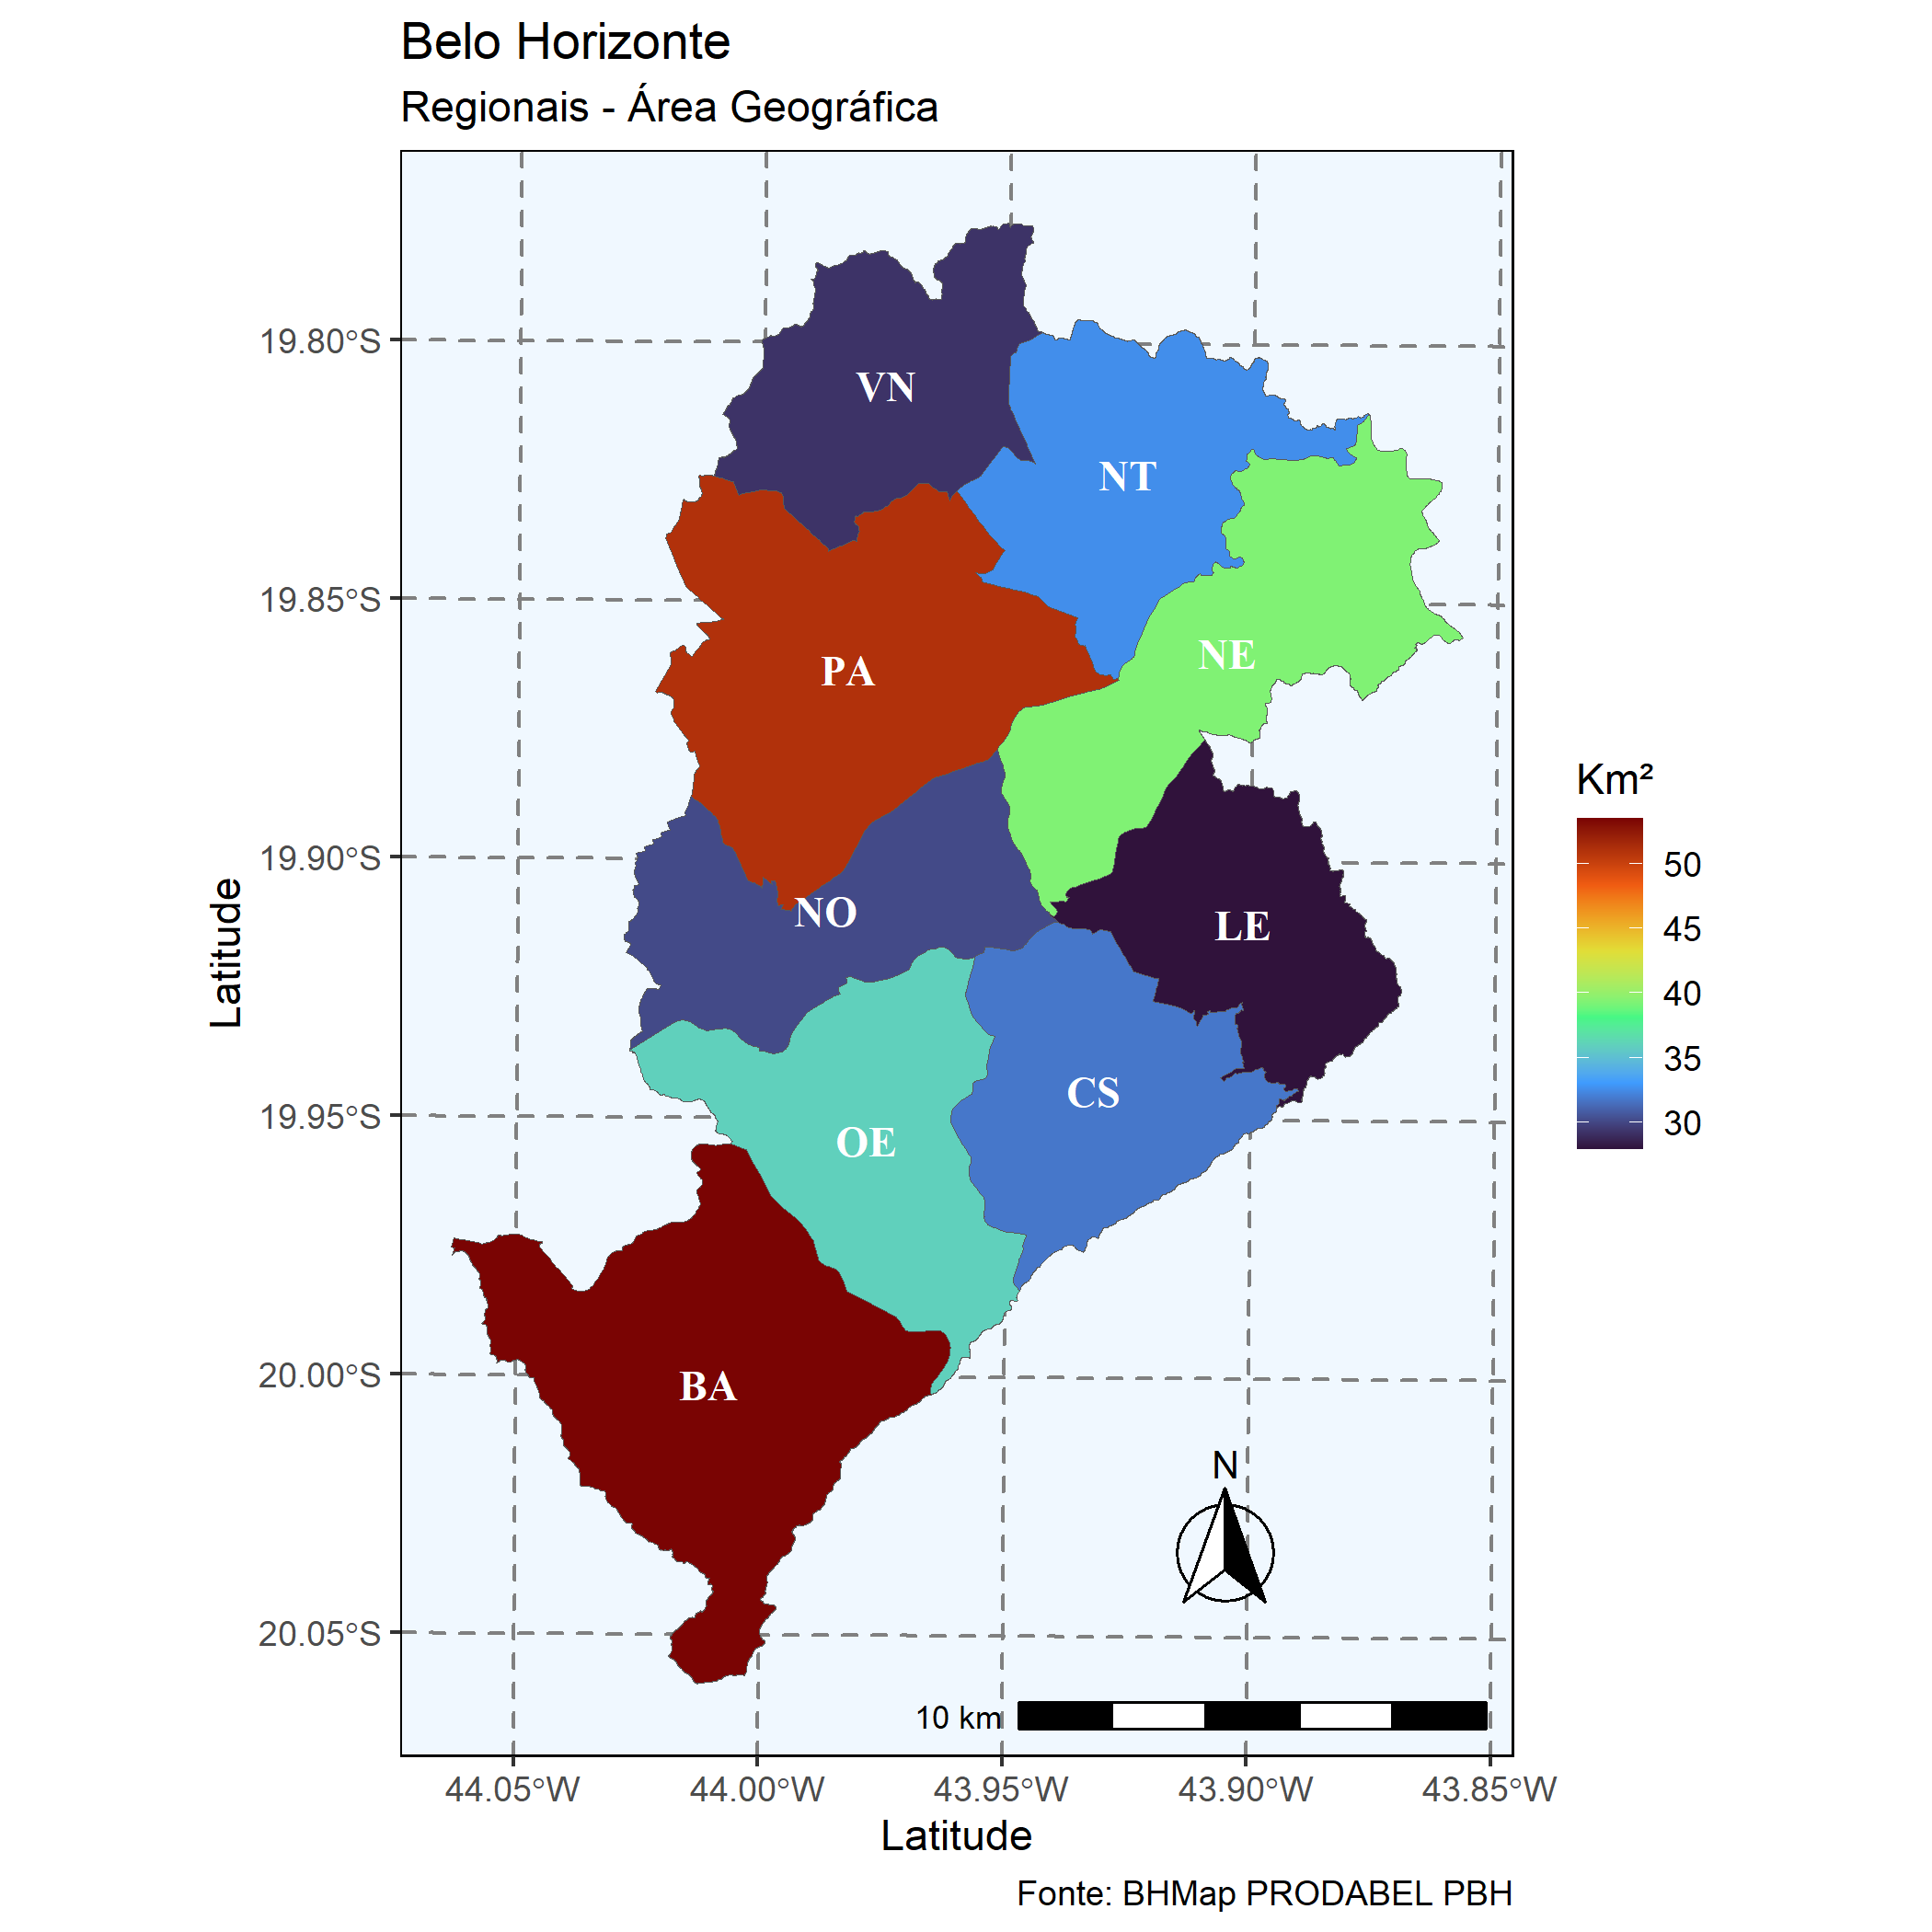
\includegraphics[scale=0.30]{imagens/area.png}
            \end{figure}
        \end{column}
        \begin{column}{7cm}
            \begin{figure}[!htbp]
                \centering
       	    %\caption{População das Regionais de Belo Horizonte}
       	    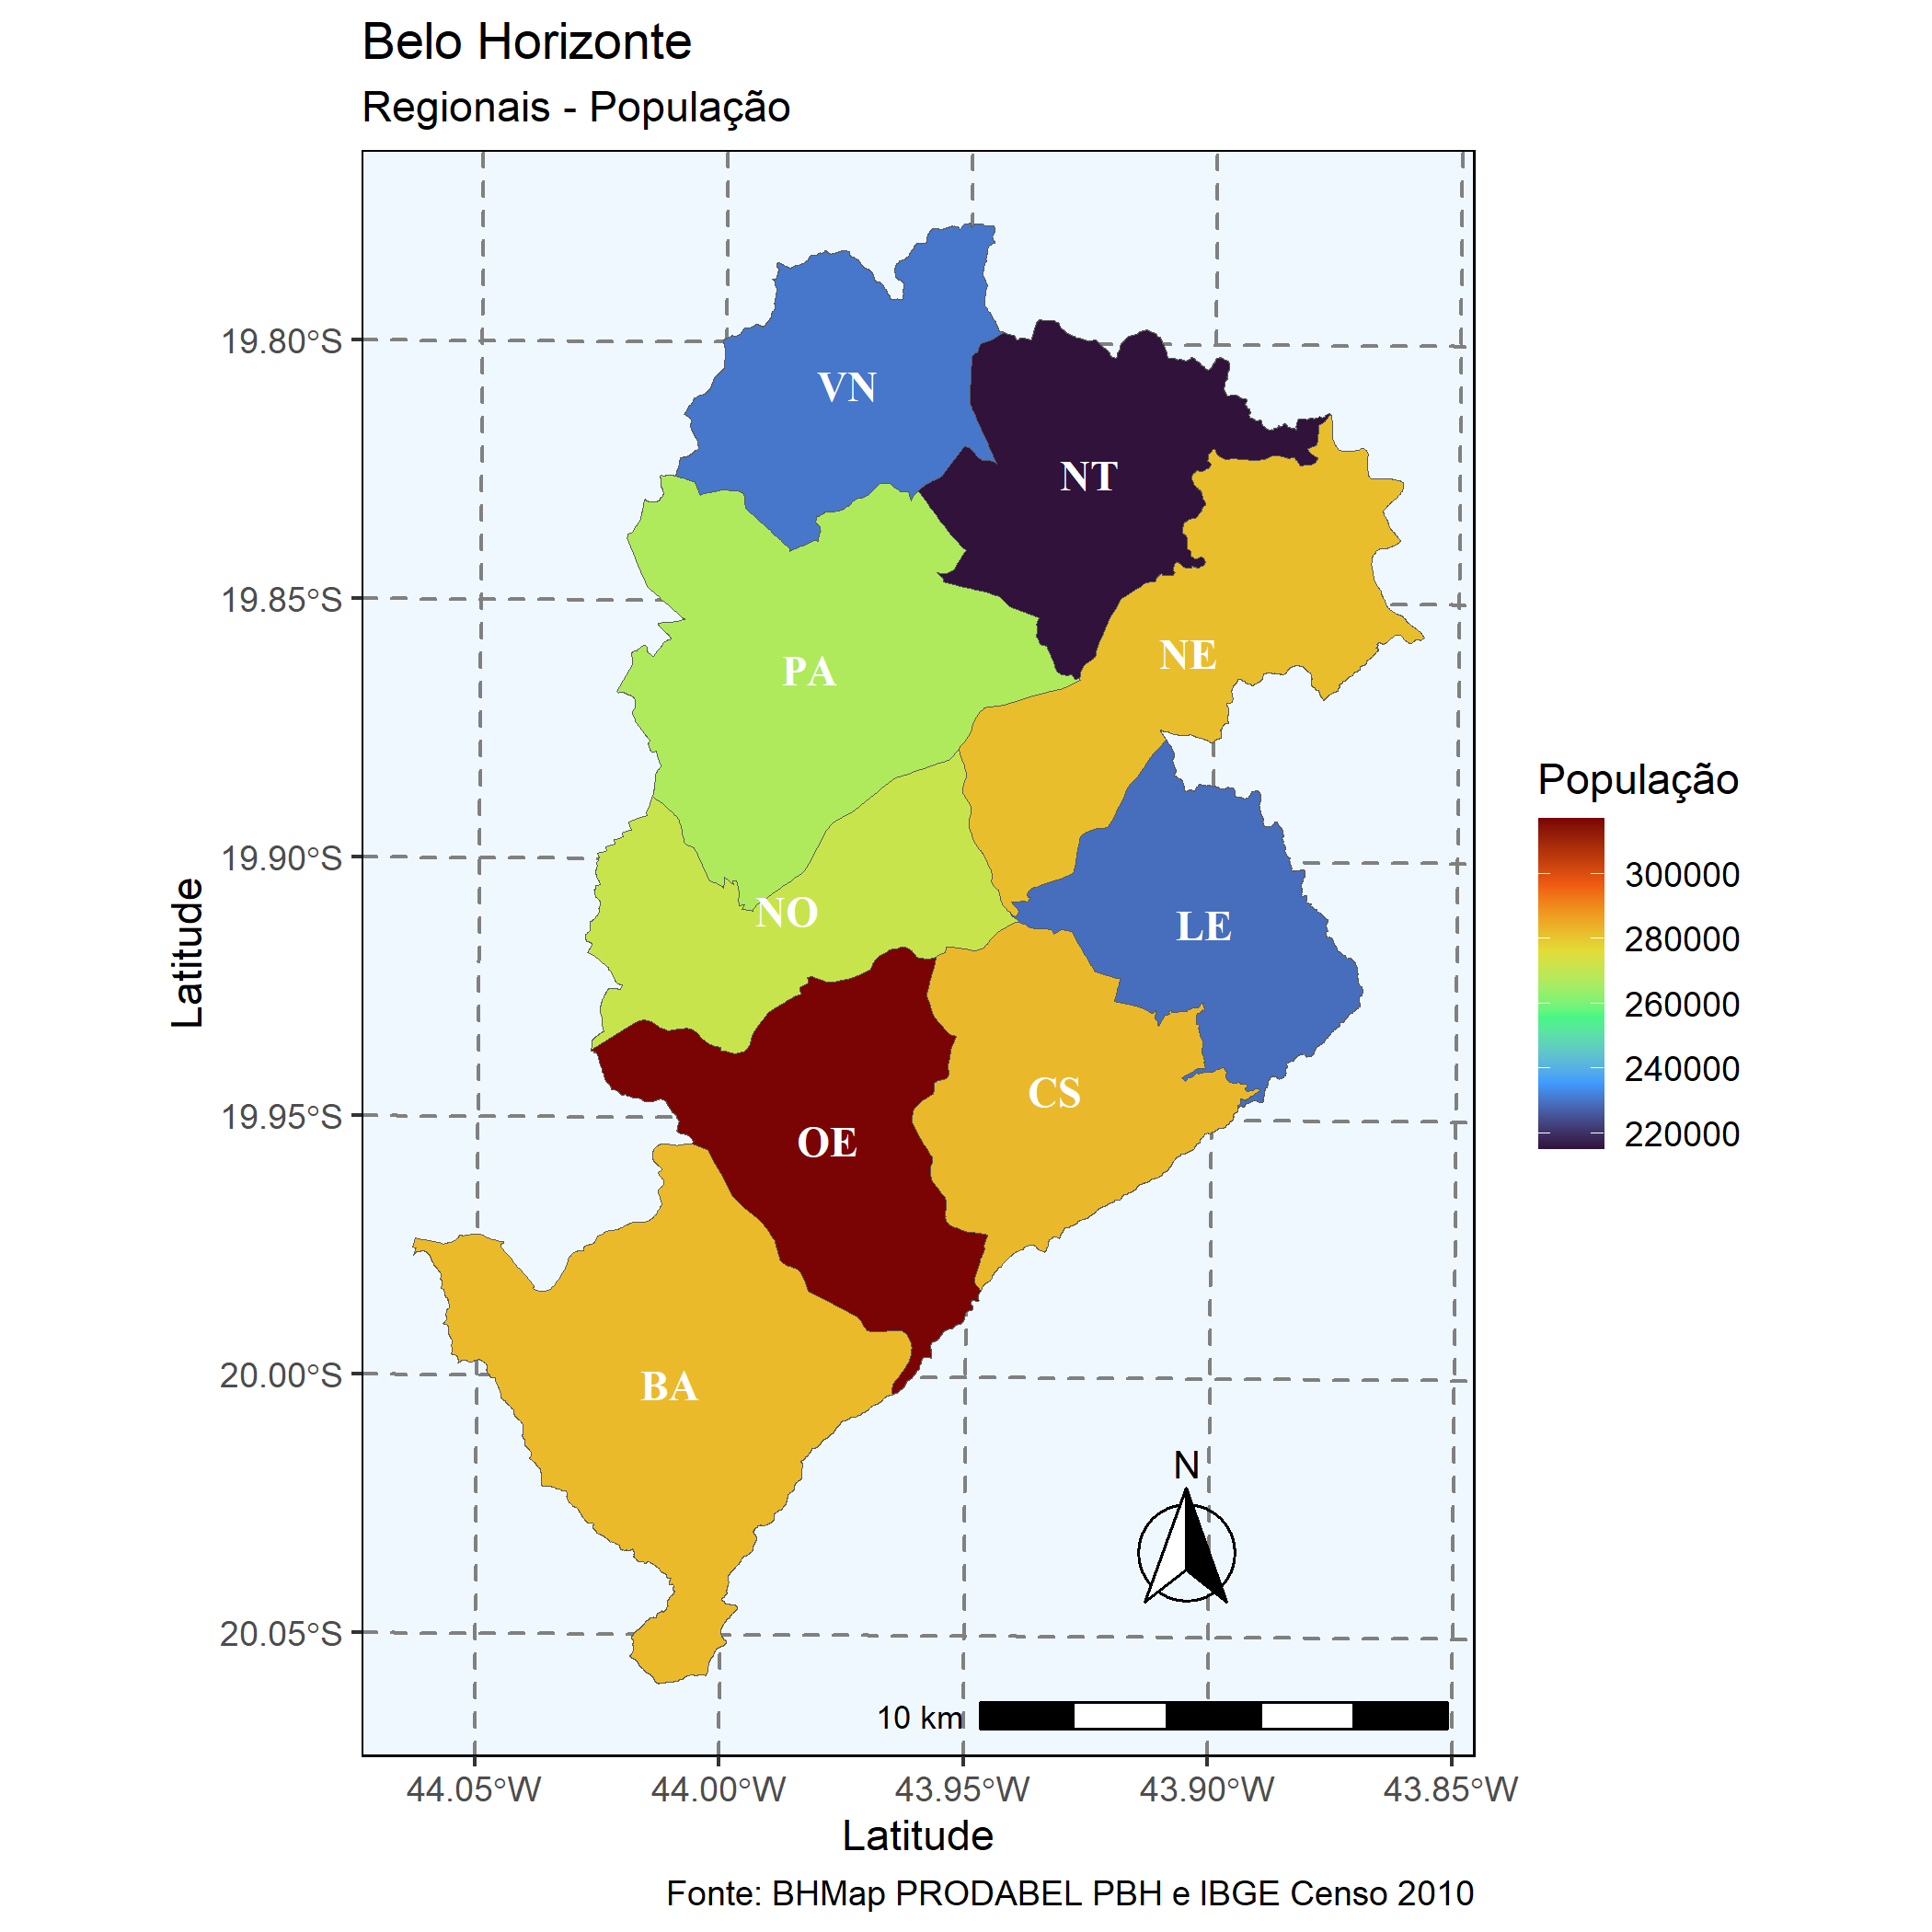
\includegraphics[scale=0.30]{imagens/populacao.png}
            \end{figure}
        \end{column}
    \end{columns}
\end{frame}


\begin{frame}

    \frametitle{Mapas das Regionais}

    \begin{columns}[t]
        \begin{column}{7cm}
            \begin{figure}[!htbp]
                \centering
       	    %\caption{Área das Regionais de Belo Horizonte}
       	    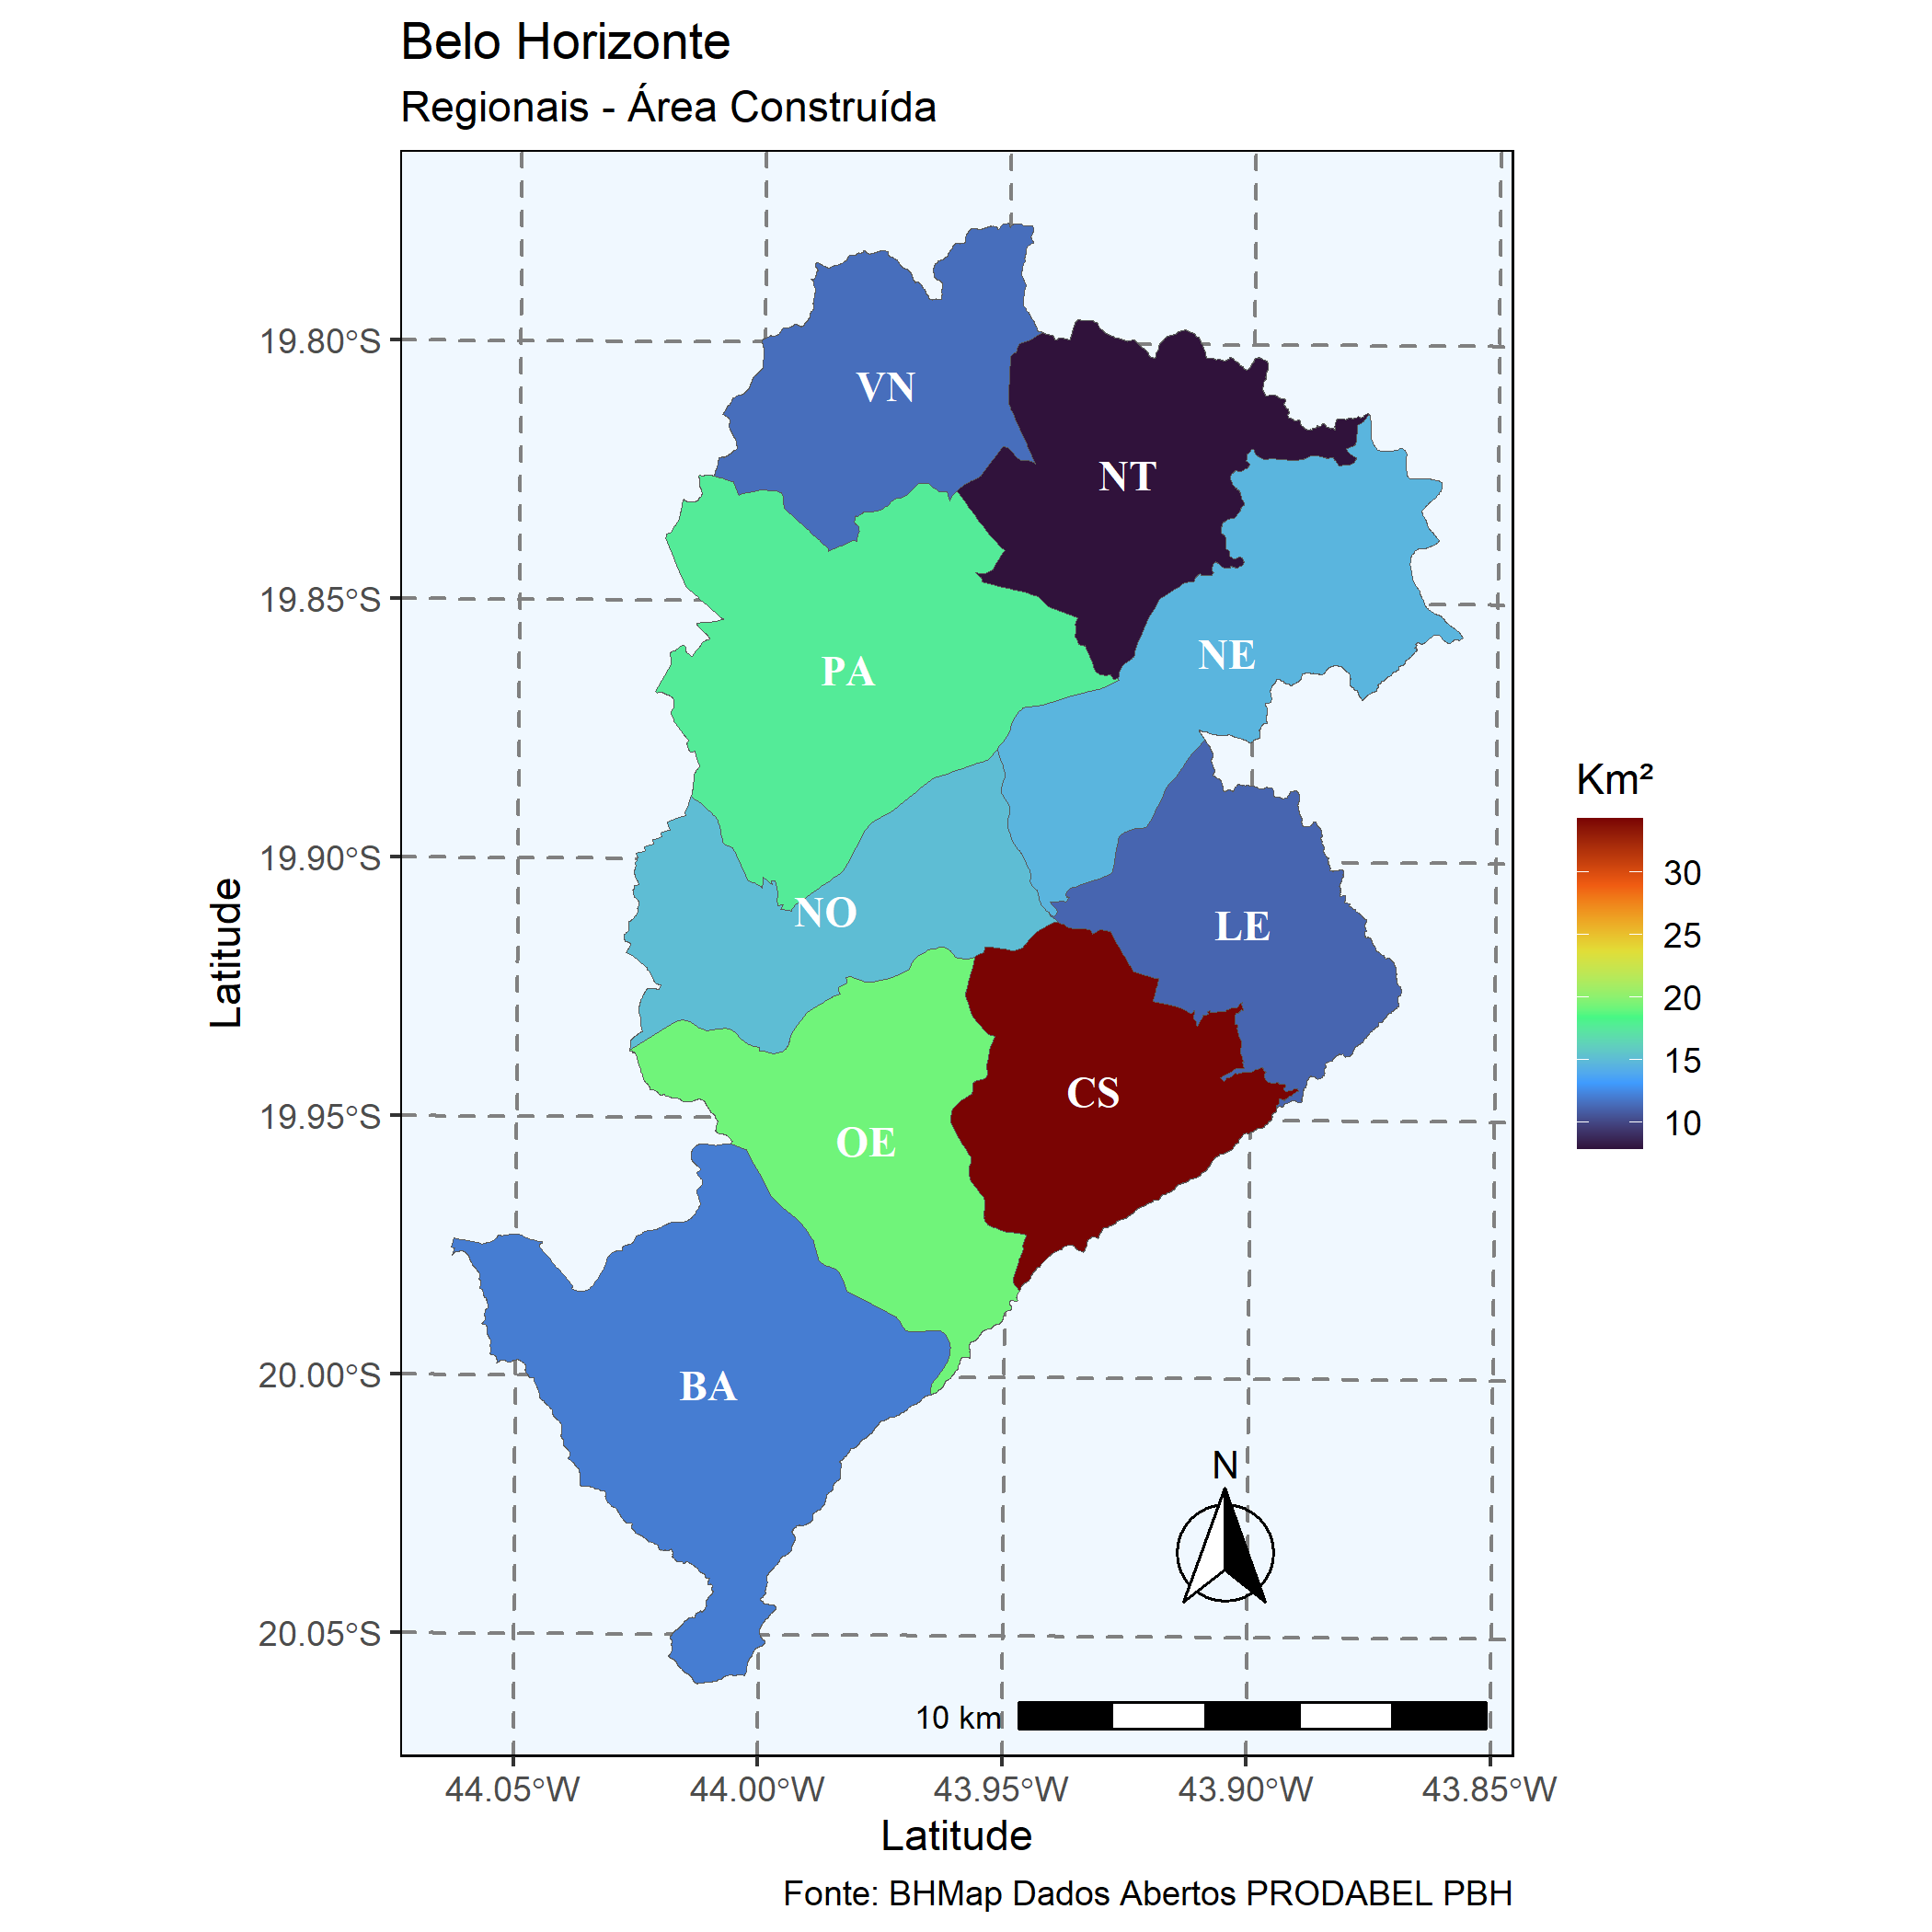
\includegraphics[scale=0.30]{imagens/area_construida.png}
            \end{figure}
        \end{column}
        \begin{column}{7cm}
            \begin{figure}[!htbp]
                \centering
       	    %\caption{População das Regionais de Belo Horizonte}
       	    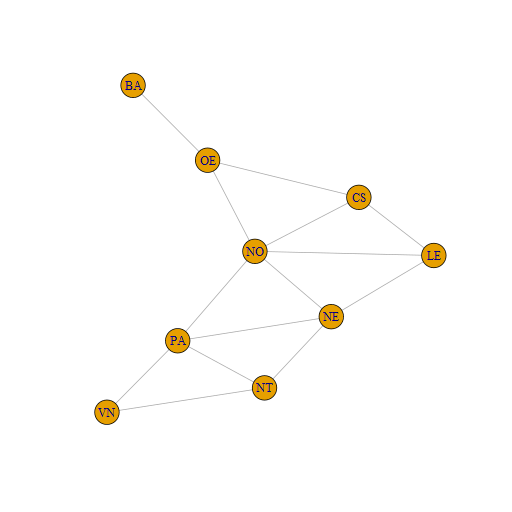
\includegraphics[scale=0.35]{imagens/grafo.png}
            \end{figure}
        \end{column}
    \end{columns}
\end{frame}


\subsection{Características}

\begin{frame}

    \frametitle{Coleta de Lixo}
    \begin{figure}[!htbp]
                \centering
       	    %\caption{População das Regionais de Belo Horizonte}
       	    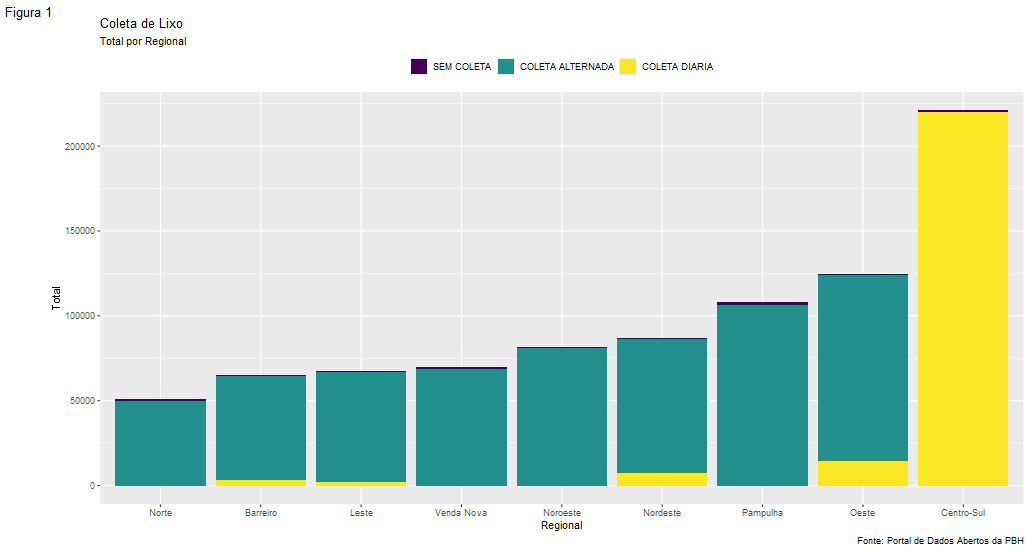
\includegraphics[scale=0.35]{imagens/coleta.png}
            \end{figure}

\end{frame}
\begin{frame}

    \frametitle{Perfil}
    \begin{figure}[!htbp]
                \centering
       	    %\caption{População das Regionais de Belo Horizonte}
       	    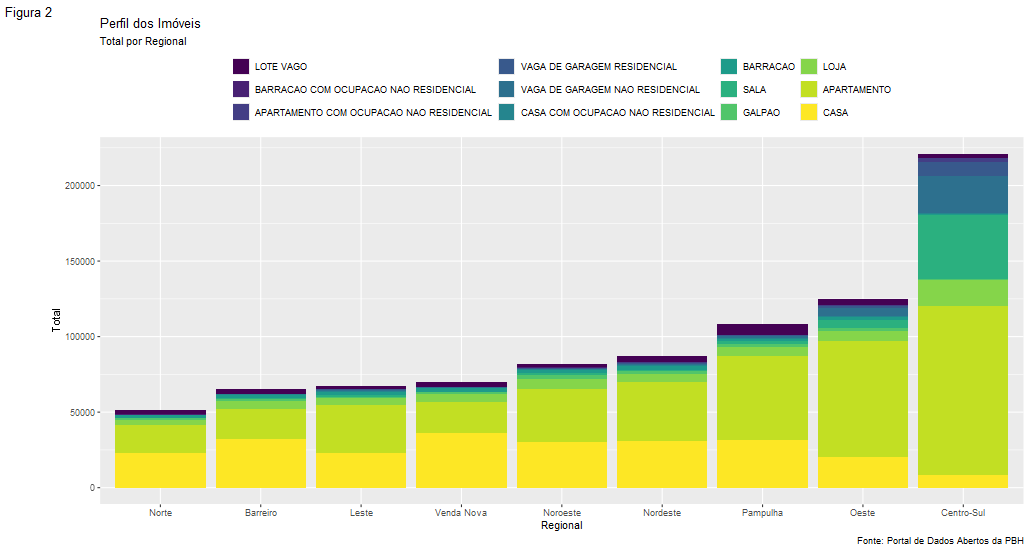
\includegraphics[scale=0.35]{imagens/perfil.png}
            \end{figure}

\end{frame}

\begin{frame}

    \frametitle{Ocupação}
    \begin{figure}[!htbp]
                \centering
       	    %\caption{População das Regionais de Belo Horizonte}
       	    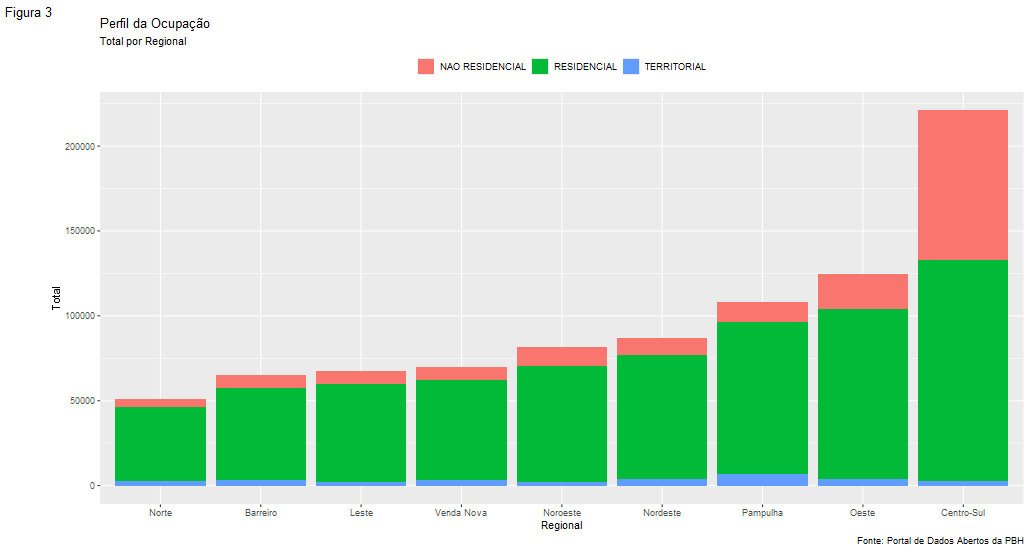
\includegraphics[scale=0.35]{imagens/ocupacao.png}
            \end{figure}

\end{frame}

\begin{frame}

    \frametitle{Qualidade do Acabamento}
    \begin{figure}[!htbp]
                \centering
       	    %\caption{População das Regionais de Belo Horizonte}
       	    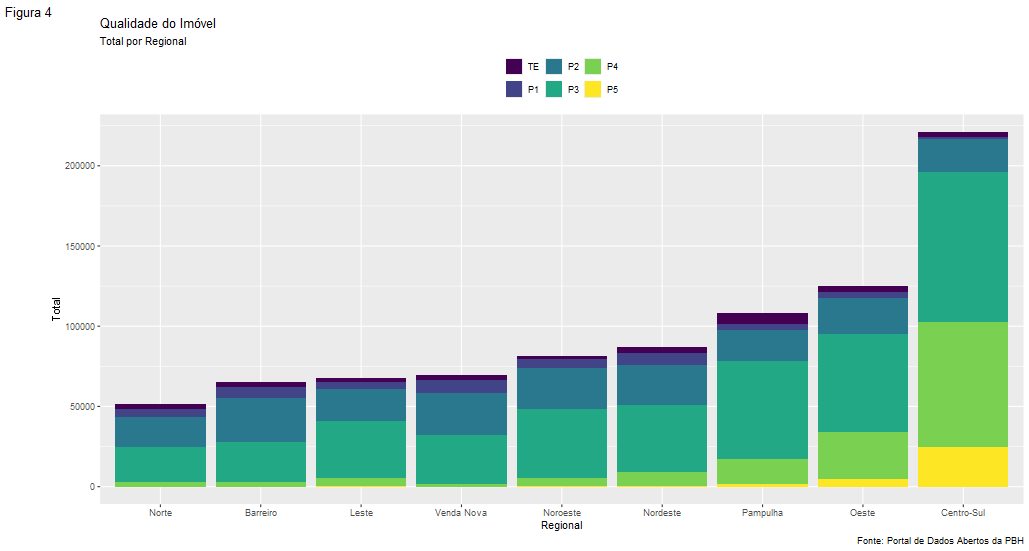
\includegraphics[scale=0.35]{imagens/acabamento.png}
            \end{figure}

\end{frame}